\section{Projekt systemu}
\author{Filip Czajkowski}
\subsection{Cele systemu}
\paragraph{}Wytworzony system miał na celu umożliwić wygenerowanie rozkładu zajęć na podstawie dostępnych danych opisujących daną placówkę edukacyjną. Poprzez zastosowanie kilku algorytmów do rozwiązania tego problemu, umożliwiać miał porównanie ich wydajności. System miał także udostępniać wizualną prezentację powstałego planu dla danego programu nauczania, aby móc go ocenić pod kątem praktycznego zastosowania.
\subsection{Wymagania}
\paragraph{}Powstały system miał narzucone następujące ograniczenia techniczne:
\begin{itemize}
\item Aplikacja po stronie klienta jest dostępna z poziomu przeglądarki z obsługą JavaScript i wymaga jedynie aktywnego połączenia z serwerem.
\item Aby uruchomić algorytmy po stronie serwera, potrzebne jest posiadanie zainstalowanych następujących komponentów:
\begin{enumerate}
\item kompilator języka \emph{Python 2.7}
\item środowisko wytwórcze aplikacji internetowych w języku Python \emph{Django 1.6}
\item system rozproszonego kolejkowania zadań \emph{Celery 3.1}
\item system komunikacji kolejek systemowych \emph{RabbitMQ 3}
\item obsługa bazy danych \emph{SQLite v.3}
\item obsługa biblioteki JavaScript \emph{ExtJS 4.2}
\item obsługa stylów i widoków w języku HTML \emph{Bootstrap 3.0.3}.
\end{enumerate}
\end{itemize}
\paragraph{}Wymagania funkcjonalne:
\begin{itemize}
\item Konieczność logowania się w celu korzystania z systemu.
\item Możliwość wywołania procesu generowania planu zajęć z koniecznością wyboru algorytmu.
\item Możliwość ustawienia limitu czasowego na czas działania procesu.
\item Pobieranie z pliku tekstowego wedle ustalonego wzorca zestawu ograniczeń opisujących potrzeby rozkładu zajęć.
\item Podgląd listy wykonanych wcześniej zadań oraz stanu uruchomionych obecnie procesów.
\item Wybranie z listy zadań konkretnego przypadku i odczytanie informacji o przyporządkowanych zajęciach do poszczególnych kursów.
\item W widoku zakończonego zadania możliwość wybrania z listy programów nauczania dowolnego z nich i przedstawienie wszystkich przydzielonych kursów w formie tabeli.
\item Możliwość zapisania na dysku wygenerowanego zestawu planów do arkuszy w pliku w formacie \emph{.csv}.
\end{itemize}
\subsection{Zastosowanie}
\paragraph{}Wytworzony system może mieć zastosowanie dwojakie. Pierwsze z nich należy do pola naukowo - badawczego i szczególnie pod tym kątem było projektowane. Dotyczy ono samego zagadnienia układania planu zajęć, umożliwia porównanie zastosowanych trzech metod pod kątem np. czasu pracy czy samej efektywności procesu. Drugim obszarem zastosowań jest platforma biznesowa, choć dość ograniczona w tym przypadku. Posiadając dane na temat jakiejś placówki dydaktycznej w odpowiednim formacie będziemy mogli ułożyć dla niej realny rozkład zajęć. Udostępniany przez system sposób wizualizacji wynikowego planu umożliwia poddanie go trafnej ocenie przydatności przez człowieka.
\subsubsection{Przypadki użycia}
\begin{itemize}
\item{\textbf{Aktorzy}} - Wszyscy mogą korzystać z systemu w ten sam sposób, więc istnieje jeden aktor, podstawowy użytkownik systemu. Natomiast aby przeprowadzić jakąkolwiek operację konieczne jest zalogowanie się na wcześniej utworzone konto.
\end{itemize}
\paragraph{}Przypadki użycia systemu, pod których kątem zostały zdefiniowane wymagania i wytworzony cały system prezentują się następująco.
\begin{center}
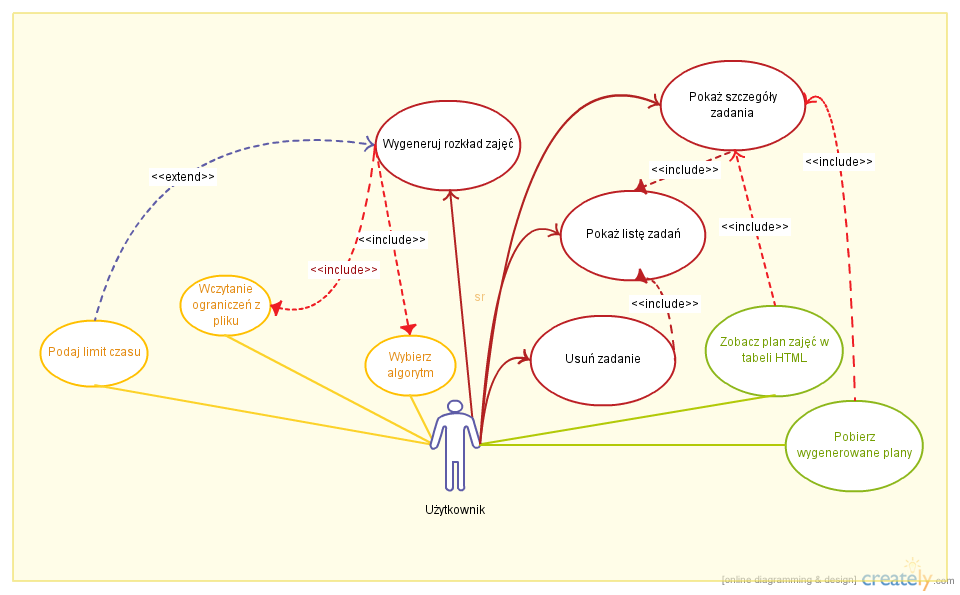
\includegraphics[width=0.8\textwidth]{img/InzynierkaUseCase.png}
\end{center}
\subsection{Architektura systemu}
\paragraph{} Ogólna architektura systemu oparta jest na modelu klient - serwer.
\begin{center}
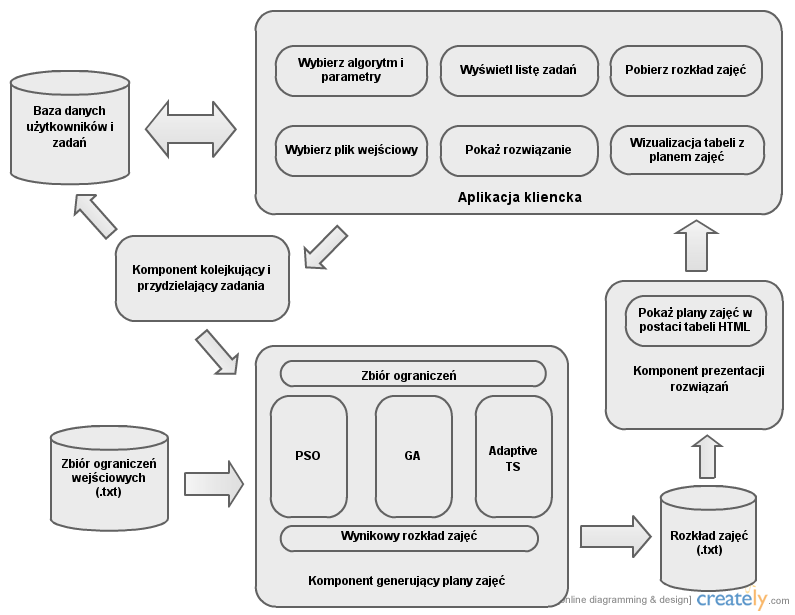
\includegraphics[width=0.8\textwidth]{img/ComponentsDiagram.png}
\end{center}
\subsection{Rozwiązania implementacyjne}
\paragraph{Komunikacja} - schemat komunikacji w systemie po stronie serwera podczas wywołania zadania generującego plan prezentuje poniższy diagram.
\begin{center}
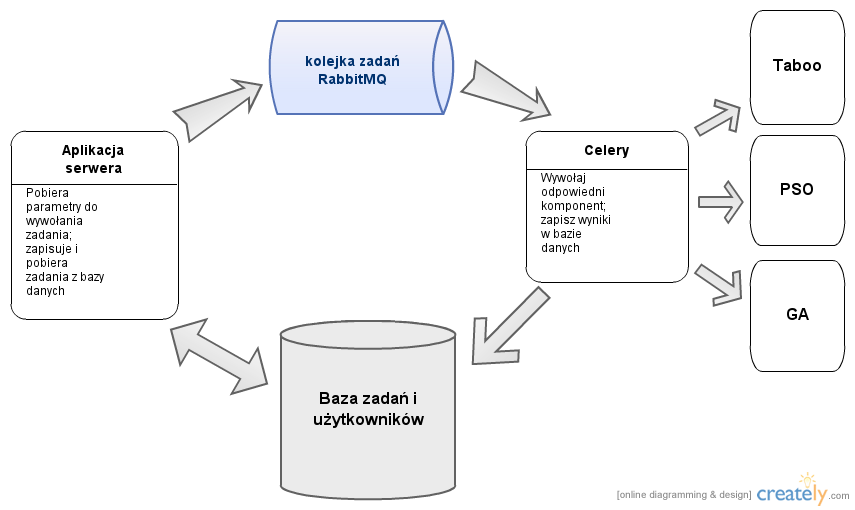
\includegraphics[width=0.8\textwidth]{img/SystemCommunication.png}
\end{center}
Gdy użytkownik prześle plik wejściowy i parametry wykonania, następuje wywołanie procedury wytworzenia planu zajęć. Aplikacja serwera przekazuje wiadomość o potrzebie wykonania zadania wraz z informacją jaki algorytm wywołać i gdzie znajduje się plik wejściowy. Zlecone zadania są zapamiętywane w kolejce systemowej. Następnie, gdy obiekt wywołujący zadania jest wolny, podbiera z kolejki zadanie i następnie wywołuje odpowiedni komponent wskazany przez typ stosowanego algorytmu. Po wykonaniu zadania zapisuje zwrócony plan zajęć do pliku i dodaje w bazie danych wpis o kolejnym zakończonym zadaniu. Dzięki tej informacji aplikacja kliencka może później pobrać informacje o wygenerowanym planie.
\paragraph{}W celu zapisywania wygenerowanych planów, została stworzona  na serwerze określona struktura plików. Istnieją dwa foldery \emph{input} oraz \emph{output}, w których składowane są pliki odpowiednio z danymi wejściowymi dla algorytmu oraz z planem wynikowym. Rozróżniane są dzięki swojej nazwie, która odpowiada numerowi identyfikującemu zadanie w bazie danych.
\paragraph{} Implementacja samych komponentów generujących plan wedle trzech algorytmów powstawała przy współudziale czterech osób. Stąd współdzielą one część kodu, ale też niektóre stosowane struktury są odmienne. Szczegółowy opis struktur poszczególnych rozwiązań zawiera się w rozdziale Implementacja (referencja!!!!!).